% override specific chktex warnings

% chktex-file 1 - ignore commands followed by a space, e.g. \\ new line here
% chktex-file 3 - enclose previous parentheses wit {}
% chktex-file 9 - sometimes messes up with ( and {
% chktex-file 36 - put a space in front of parentheses
% chktex-file 45 - don't use $$ instead of \[, etc
% chktex-file 46 - don't use $ instead of \(, etc


\documentclass[10pt, oneside]{amsart}
% \usepackage[showboxes]{textpos}

\usepackage[absolute,overlay]{textpos}
\setlength{\TPHorizModule}{1.0cm}
\setlength{\TPVertModule}{\TPHorizModule}
\textblockorigin{0.0cm}{0.0cm}  %start all at upper left corner

\usepackage{amsmath}
\usepackage{amsthm}
\usepackage{amsfonts}
\usepackage{amssymb}
\usepackage{mathpazo}
\usepackage{booktabs}
\usepackage[usenames,x11names]{xcolor}
\usepackage{tikz}
\usepackage{textcomp}
\usepackage[letterpaper]{geometry}
\geometry{verbose,tmargin=0.5in,bmargin=0.5in,lmargin=1in,rmargin=0.5in}
\usepackage{multicol}
\usepackage{bm}
\usepackage{comment}
\usepackage{cancel}
\usepackage{array}
\usepackage{gensymb}
\usepackage{enumerate}
\usepackage[many]{tcolorbox}

\pagestyle{plain}
\raggedright
\renewcommand{\familydefault}{\sfdefault}
\setlength{\parskip}{\medskipamount}
\setlength{\columnsep}{1cm}

\everymath{\displaystyle}
\setlength{\parskip}{\bigskipamount}
\definecolor{structure}{RGB}{100,100,100}
% counter for resuming enumerated list numbers
\newcounter{resumeenumi}
\newcommand{\suspend}{\setcounter{resumeenumi}{\theenumi}}
\newcommand{\resume}{\setcounter{enumi}{\theresumeenumi}}

\newcommand\lb{\linebreak}
\newcommand\pars{\par\smallskip}
\newcommand\parm{\par\medskip}
\newcommand\parb{\par\bigskip}

\makeatletter
\providecommand{\gettikzxy}[3]{%
	\tikz@scan@one@point\pgfutil@firstofone#1\relax
	\edef#2{\the\pgf@x}%
	\edef#3{\the\pgf@y}%
}
\makeatother



% full width colored block but color specifiable
%\cb[body bg strength]{header bg}{header text}{body text}
\newcommand{\cb}[4][15]{
	\setbeamercolor{block title}{bg = #2}
	\setbeamercolor{block body}{bg = #2!#1}
	\setbeamercolor{item projected}{bg=#2, fg=white}
	\begin{center}
		\begin{block}{#3}
			#4
		\end{block}
	\end{center}
}

% colored block with width specified
% \cbw[body bg strength]{header bg}{width}{header text}{body text}
\newcommand{\cbw}[5][15]{
	\begin{center}
		%\vspace{-0.35cm}
		\begin{minipage}{#3\textwidth}
			\setbeamercolor{block title}{bg= #2}
			\setbeamercolor{block body}{bg= #2!#1}
			\setbeamercolor{item projected}{bg=#2, fg=white}
			\begin{block}{#4}
				\raggedright
				#5
			\end{block}
		\end{minipage}
	\end{center}
}

% centered minipage with text \raggedright
%\cmini[width]{content}
\newcommand{\cmini}[2][0.8]{
	\begin{center}
		\begin{minipage}{#1\columnwidth}
			\raggedright
			#2
		\end{minipage}
	\end{center}
}

%left flushed minipage
\newcommand{\mini}[2][0.8]{
	\begin{minipage}{#1\columnwidth}
		\raggedright
		#2
	\end{minipage}
}

%left flushed minipage, top aligned
\newcommand{\minit}[2][0.8]{
	\begin{minipage}[t]{#1\columnwidth}
		\raggedright
		#2
	\end{minipage}
}

%left flushed minipage
% \newcommand{\miniT}[2][0.8]{
%  \begin{minipage}[T]{#1\columnwidth}
%   \raggedright
%   #2
%  \end{minipage}
% }

%left flushed minipage
\newcommand{\minib}[2][0.8]{
	\begin{minipage}[b]{#1\columnwidth}
		\raggedright
		#2
	\end{minipage}
}

\newcommand{\cfig}[2][1]{% centred, scaled graphic
	\begin{center}
		\includegraphics[scale=#1]{#2}
	\end{center}
}
% figure with tight border for photos
% \cfigb[saitMaroon]{borderwidth with unit}{scale}{image}
\newcommand{\cfigb}[4][structure]{
	% \usepackage{adjustbox}
	\setlength{\fboxrule}{1pt}
	\begin{center}
		\includegraphics[scale=#3, cframe= #1 #2]{#4}
	\end{center}
}

\newcommand{\imgbox}[3]{
	% \setlength{\fboxsep}{12pt}
	\includegraphics[scale=#1, cframe= structure #3]{#2}
}

% \imgboxbg[bg color=white]{scale}{path/to/img}{border color}{border, e.g. 2pt}{margin, e.g. 4pt}
\newcommand{\imgboxbg}[6][white]{
	\setlength{\fboxrule}{#5}
	\setlength{\fboxsep}{#6}
	\centering
	\fcolorbox{#4}{#1}{\includegraphics[scale=#2]{#3}}
}

\newcommand{\fig}[2][1]{% scaled graphic
	\includegraphics[scale=#1]{#2}
}

% centred framed  box black border
%\cbox[width]{content}
\newcommand{\cbox}[2][0.9]{% framed centered  box
	\setlength\fboxsep{0.042\columnwidth}
	\setlength\fboxrule{0.0015\columnwidth}
	\begin{center}
		\fcolorbox{black}{white}{
			\vspace{-0.5cm}
			\begin{minipage}{#1\columnwidth}
				\raggedright
				#2
			\end{minipage}
		}
	\end{center}
	\setlength\fboxsep{0cm}
}



\newtcolorbox{mybox}[1][]
{
	colback=white,
	top=0.25cm,
	bottom=0.25cm,
	left=0.25cm,
	right=0.25cm,
	colframe=structure,
	fonttitle=\bfseries,
	enhanced, drop fuzzy shadow,
	% attach boxed title to top left={yshift=-2mm, xshift=5mm},
	attach boxed title to top left={yshift=-2mm, xshift=5mm}, colbacktitle=structure!80!white, #1}

\newtcolorbox{plainbox}[1][]{colback=white, sharp corners, top=0.125cm, bottom=0.125cm, left=0pt, right=0pt, boxrule=0.5pt,colframe=structure,fonttitle=\bfseries, colbacktitle=structure, arc=0mm, #1}
%
\newtcbtheorem{myexam}{Example}%
{
	enhanced,
	colback=white,
	top=0.375cm,
	bottom=0.25cm,
	left=0.375cm,
	right=0.375cm,
	colframe=structure,
	fonttitle=\bfseries,
	drop fuzzy shadow,
	%description font=\mdseries\itshape,
	attach boxed title to top left={yshift=-2mm, xshift=5mm},
	colbacktitle=structure!80!white
	}{exam}% then \pageref{exer:theoexample} references the theo

\newcommand{\myexample}[2][red]{
	% \tcb\tcbset{theostyle/.style={colframe=red,colbacktitle=yellow}}
	\begin{myexam}{}{}
		\raggedright
		#2
	\end{myexam}
	% \tcbset{colframe=structure,colbacktitle=structure}
}

\newtcbtheorem{myexer}{Exercise}%
{
	enhanced,
	colback=white,
	top=0.375cm,
	bottom=0.25cm,
	left=0.375cm,
	right=0.375cm,
	colframe=structure,
	fonttitle=\bfseries,
	drop fuzzy shadow,
	%description font=\mdseries\itshape,
	attach boxed title to top left={yshift=-2mm, xshift=5mm},
	colbacktitle=structure!80!white
	}{exer}

\newcommand{\myexercise}[2][red]{
	% \tcb\tcbset{theostyle/.style={colframe=red,colbacktitle=yellow}}
	\begin{myexer}{}{}
		\raggedright
		#2
	\end{myexer}
	% \tcbset{colframe=structure,colbacktitle=structure}
}


\begin{document}

\thispagestyle{empty}
\vspace{-7cm}
\centering
\textbf{\Large Module 8: Hazen Williams Equation and Equivalent Pipes (CIVL 318)}
\par\medskip
\centering
\cbox[0.8]{
	\centering
	\textbf{\large Hazen-Williams Equations}
	\[
		Q = \frac{C\,D^{2.63}\left(\frac{h_L}{L}\right)^{0.54}}{279000},\qquad
		h_L = L\,\left(\frac{279000\,Q}{C\,D^{2.63}}\right)^{1.852},\qquad
		D = \left(\frac{279000\,Q}{C\,\left(\frac{h_L}{L}\right)^{0.54}}\right)^{0.3802}
	\]
}
\cbox[0.7]{
	\centering
	\textbf{\Large Equivalent-Length Ratios for Fittings}
	\parb
	\begin{tabular}{r >{$}r<{$} >{$}l<{$} >{$}c<{$} }
		\toprule
		\text{Type}                                                    & \quad & L_e/D \\
		\midrule
		\addlinespace
		Globe valve --- fully open                                     &       & 340   \\
		\addlinespace
		Angle valve --- fully open                                     &       & 150   \\
		\addlinespace
		Gate valve --- fully open                                      &       & 8     \\
		\addlinespace
		--- $3/4$ open                                                 &       & 35    \\
		\addlinespace
		--- $1/2$ open                                                 &       & 160   \\
		\addlinespace
		--- $1/4$ open                                                 &       & 900   \\
		\addlinespace
		Check valve --- swing type                                     &       & 100   \\
		\addlinespace
		Check valve --- ball type                                      &       & 150   \\
		\addlinespace
		Butterfly valve --- fully open --- 2-8''                       &       & 45    \\
		\addlinespace
		--- 10-14''                                                    &       & 35    \\
		\addlinespace
		--- 16-24''                                                    &       & 25    \\
		\addlinespace
		Foot valve --- poppet disc type                                &       & 420   \\
		\addlinespace
		Foot valve --- hinged disc type                                &       & 75    \\
		\addlinespace
		$90\degree$ standard elbow                                     &       & 30    \\
		\addlinespace
		$90\degree$ long radius elbow                                  &       & 20    \\
		\addlinespace
		$90\degree$ street elbow                                       &       & 50    \\
		\addlinespace
		$45\degree$ standard elbow                                     &       & 16    \\
		\addlinespace
		$45\degree$ street elbow                                       &       & 26    \\
		\addlinespace
		Close return bend                                              &       & 50    \\
		\addlinespace
		Standard tee --- flow through run                              &       & 20    \\
		\addlinespace
		Standard tee --- flow through branch                           &       & 60    \\
		\addlinespace
		Gradual enlargement --- $15^\circ$ cone angle                  &       & 8     \\
		\addlinespace
		Gradual enlargement --- $20^\circ$ cone angle                  &       & 15    \\
		\addlinespace
		Gradual enlargement --- $30^\circ$ cone angle                  &       & 23    \\
		\addlinespace
		Gradual reduction --- $15^\circ\text{ to }40^\circ$ cone angle &       & 2     \\
		\addlinespace
		Pipe entrance --- inward projecting                            &       & 50    \\
		\addlinespace
		Pipe entrance --- square                                       &       & 25    \\
		\addlinespace
		Pipe entrance --- rounded                                      &       & 10    \\
		\addlinespace
		Venturi meter                                                  &       & 100   \\
		\addlinespace
	\end{tabular}
}
\raggedright
\newpage



%%%%%%%%%%%%%%%%%%%%%%%%%%%%%%%%%%%%%%%%%%%%%%%%%%%%%%%%%%%%%%%%%%%%%%%%%%%%%%%%%%%%%%%%%%%%%%%%%%%%%%%%%


\begin{myexam}{}{}
	\cmini[0.7]{
		For the pipeline shown, calculate the pressure at $B$, given that the pressure at $A$ is
		$700\,\text{kPa}$.\parm
		The pipes are cement-lined Hyprescon with a diameter of $400\,\text{mm}$ and a roughness coefficient of $C=140$. Flow through the system is $200\,\text{L/s}$.
		\parm
		Elevations are as indicated.
		\cfig[0.5]{../../figs/08HWEquivPipe/HW1}
	}
\end{myexam}

\mini[0.5]{
	\Large
	\parb
	\textbf{Solution}:\parb
	First, apply the Hazen-Williams:
	\cbox[0.9]{
		\begin{align*}
			h_{L_{AB}} & = L\,\left(\frac{279000\,Q}{C\,D^{2.63}}\right)^{1.852}                    \\
			           & = 1000\,\left(\frac{279000\times 200}{140\times 400^{2.63}}\right)^{1.852} \\
			           & = 4.9903\,\text{m}                                                         
		\end{align*}
	}
	\parb
	Now, apply the GEE:
	
	\cbox[0.9]{
		\begin{align*}
			\frac{P_A}{\gamma} + \cancel{z_A} + \cancel{\frac{v_A^2}{2g}} -h_L & = \frac{P_B}{\gamma} + \cancel{z_B} + \cancel{\frac{v_B^2}{2g}} \\
			\frac{700}{9.81}  -4.9903                                          & = \frac{P_B}{9.81}                                              \\\\
			P_B                                                                & = 651.05\,\text{kPa}                                            \\
			\bm{P_B}                                                           & =       \bm{651}\,\textbf{kPa}                                  
		\end{align*}
	}
}

\newpage

%%%%%%%%%%%%%%%%%%%%%%%%%%%%%%%%%%%%%%%%%%%%%%%%%%%%%%%%%%%%%%%%%%%%%%%%%%%%%%%%%%%%%%%%%%%%%%%%%%%%%%%%%


\begin{myexer}{}{}
	\cmini{
		For the pipeline shown, calculate the pressure at $C$ and $D$, given that the pressure at $A$ is
		$700\,\text{kPa}$.\parm
		The pipes are cement-lined Hyprescon with a diameter of $400\,\text{mm}$ and a roughness coefficient of $C=140$. Flow through the system is $200\,\text{L/s}$.
		\parm
		Elevations are as indicated.
		
		\cfig[0.5]{../../figs/08HWEquivPipe/HW1}
	}
\end{myexer}

\Large\parb
\textbf{Solution}:\parb
\normalsize
\minit[0.5]{
	First, apply the Hazen-Williams:
	
	
	\cbox[0.9]{
		\large
		\begin{align*}
			h_{L_{BC}} & = L\,\left(\frac{279000\,Q}{C\,D^{2.63}}\right)^{1.852}                   \\
			           & = 800\,\left(\frac{279000\times 200}{140\times 400^{2.63}}\right)^{1.852} \\
			           & = 3.9922\,\text{m}                                                        
		\end{align*}
	}
	\parb
	\cbox[0.9]{
		\large
		\begin{align*}
			h_{L_{CD}} & = L\,\left(\frac{279000\,Q}{C\,D^{2.63}}\right)^{1.852}                    \\
			           & = 3000\,\left(\frac{279000\times 200}{140\times 400^{2.63}}\right)^{1.852} \\
			           & = 14.971\,\text{m}                                                         
		\end{align*}
	}
	
}
\hfill
\minit[0.45]{
	
	Now, apply the GEE:
	
	\cbox[0.9]{
		\large
		\begin{align*}
			\frac{P_B}{\gamma} + z_B + \cancel{\frac{v_B^2}{2g}} -h_L & = \frac{P_C}{\gamma} + z_C + \cancel{\frac{v_C^2}{2g}} \\
			\frac{651.05}{9.81}  -3.9922                              & = \frac{P_C}{9.81} + 20                                \\\\
			P_C                                                       & = 415.69\,\text{kPa}                                   \\
			\bm{P_C}                                                  & = \bm{416}\,\textbf{kPa}                               
		\end{align*}
	}
	\parb
	\cbox[0.9]{
		\begin{align*}
			\frac{P_C}{\gamma} + z_C + \cancel{\frac{v_C^2}{2g}} -h_L & = \frac{P_D}{\gamma} + z_D + \cancel{\frac{v_D^2}{2g}} \\
			\frac{415.69}{9.81}+30-14.971                             & = \frac{P_D}{9.81}                                     \\\\
			P_D                                                       & = 563.12\,\text{kPa}                                   \\
			\bm{P_D}                                                  & = \bm{563}\,\textbf{kPa}                               
		\end{align*}
	}
}

\newpage
%%%%%%%%%%%%%%%%%%%%%%%%%%%%%%%%%%%%%%%%%%%%%%%%%%%%%%%%%%%%%%%%%%%%%%%%%%%%%%%%%%%%%%%%%%%%%%%%%%%%%%%%%


\begin{myexam}{}{}
	\minit[0.475]{
		\parb\raggedright
		Water flows from a storage tank through a welded steel pipe that is 1200 m long and 350 mm in diameter, entering a
		distribution grid at point 'B'. Assume C=100. Determine:
		\begin{enumerate}
			\item The pressure at `B' when the flow is 150 L/s
			\item The maximum flow rate into the grid when the minimum allowable pressure at `B' is 400~kPa.
		\end{enumerate}
		Minor losses are negligible compared to friction losses.
	}
	\hfill
	\minit[0.475]{
		\cfig[0.5]{../../figs/08HWEquivPipe/HW2}
	}
\end{myexam}
\parb
\minit[0.475]{
	\large
	\textbf{Solution (1)}:
	\cbox{
		\begin{align*}
			h_L            & = L\,\left(\frac{279000\,Q}{C\,D^{2.63}}\right)^{1.852}                    \\
			               & = 1200\,\left(\frac{279000\times 150}{100\times 350^{2.63}}\right)^{1.852} \\
			               & = 12.561\,\text{m}                                                         \\
			v              & = \frac{Q}{A}                                                              \\
			               & = \frac{0.150}{\pi(0.350)^2/4}                                             \\
			               & = 1.5591\,\text{m/s}                                                       \\
			\frac{v^2}{2g} & = 0.12389\,\text{m}                                                        
		\end{align*}
	}
	\parb
	GEE:
	\cbox{
		\begin{align*}
			\cancelto{0}{\frac{P_A}{\gamma}} + z_A + \cancelto{0}{\frac{v_A^2}{2g}} -h_L & = \frac{P_B}{\gamma} + \cancelto{0}{z_B} + \frac{v_B^2}{2g} \\
			45 -12.561                                                                   & = \frac{P_B}{9.81} + 0.12389                                \\\\
			P_B                                                                          & = 317.01\,\text{kPa}                                        \\
			\bm{P_B}                                                                     & = \bm{317}\,\textbf{kPa}                                    
		\end{align*}
	}
	\parb
	Notice that if we recalculated the pressure at $B$ omitting the velocity head, then $P_B=318.2\,\text{kPa}$ (which is not very different from including it).
}
\hfill
\minit[0.45]{
	\textbf{Solution (2)}:\parb
	What flow/headloss will give a pressure of 400~kPa \lb at $B$?
	
	\cbox[0.9]{
		\large
		\begin{align*}
			\cancelto{0}{\frac{P_A}{\gamma}} + z_A + \cancelto{0}{\frac{v_A^2}{2g}} -h_L & = \frac{P_B}{\gamma} + \cancelto{0}{z_B} + \frac{v_B^2}{2g} \\
			45 - h_L                                                                     & = \frac{400}{9.81} + \frac{v_B^2}{2g}                       
		\end{align*}
	}
	\parb
	One equation and two unknowns! We could solve it iteratively, guessing at a flow and seeing what $P_B$ is for this flow, then trying another flow until we converge on a pressure of 400 kPa at $B$.\parm
	But the velocity head had an effect of about 0.3\% in part (1); it will be less here as we need less velocity/headloss to keep the pressure higher. So, in problems of this type, we \textbf{simply ignore the velocity head term...}
	\cbox[0.9]{
		\large
		\begin{align*}
			45 - h_L & = \frac{400}{9.81} + \cancelto{0}{\frac{v_B^2}{2g}} \\
			h_L      & = 4.2253\,\text{m}                                  
		\end{align*}
	}
	\parb
	What flow will give this headloss?
	
	\cbox[0.9]{
		\begin{align*}
			Q      & = \frac{CD^{2.63}\left(\frac{h_L}{L}\right)^{0.54}}{279000}                  \\
			       & = \frac{100\times 350^{2.63}\left(\frac{4.2253}{1200}\right)^{0.54}}{279000} \\
			       & = 83.272\,\text{L/s}                                                         \\
			\bm{Q} & =  \bm{83.3}\,\textbf{L/s}                                                   
		\end{align*}
	}
	\parb
}
\newpage

\mini[0.5]{
	Let's look at the value of the velocity head we discarded...
	
	\cbox[0.9]{
		\begin{align*}
			v              & = \frac{Q}{A}                     \\
			               & = \frac{0.083272}{\pi(0.350)^2/4} \\
			               & = 0.86551\,\text{m/s}             \\\\
			\frac{v^2}{2g} & = 0.038181\,\text{m}              
		\end{align*}
	}
	\parb
	The velocity head is small enough that we can disregard it. Any error from not omitting the headloss is negligible compared with error in estimating the $C$-value.
}

\newpage

%%%%%%%%%%%%%%%%%%%%%%%%%%%%%%%%%%%%%%%%%%%%%%%%%%%%%%%%%%%%%%%%%%%%%%%%%%%%%%%%%%%%%%%%%%%%%%%%%%%%%%%%%


\begin{myexer}{}{}
	\mini[0.425]{
		Water flows from one reservoir down to another, through a $500$ mm diameter pipe that is $2000$ m in length. The difference in elevation between the surfaces of the two reservoirs is $30$ m.
		\par\bigskip
		Determine:
		\begin{enumerate}
			\item The flow with high density polyethylene pipe (HDPE) with $C=140$
			\item The flow with welded steel with $C=100$
			\item The diameter of HDPE pipe required for a flow of $1200$ L/s
		\end{enumerate}
		Disregard minor losses.
	}
	\hfill
	\mini[0.525]{
		\cfig[0.475]{../../figs/08HWEquivPipe/HW3}
	}
\end{myexer}
\parb
\minit[0.5]{
	\textbf{\large Solution (1)}: For HDPE.
	\parm
	At the surfaces of both reservoirs, pressure and velocity head are $0$ so the GEE reduces to
	$\bm{30 - h_L = 0}$
	\cbox[0.9]{
		\large
		\begin{align*}
			Q      & = \frac{CD^{2.63}\left(\frac{h_L}{L}\right)^{0.54}}{279000}         \\
			       & = \frac{140(500)^{2.63}\left(\frac{30}{2000}\right)^{0.54}}{279000} \\
			       & =651.48\,\text{L/s}                                                 \\
			\bm{Q} & = \bm{651}\,\textbf{L/s}                                            
		\end{align*}
	}
	\parb
	\textbf{\large Solution (2)}: For welded steel,\parm
	\cbox[0.9]{
		\large
		\begin{align*}
			Q      & = \frac{CD^{2.63}\left(\frac{h_L}{L}\right)^{0.54}}{279000}         \\
			       & = \frac{100(500)^{2.63}\left(\frac{30}{2000}\right)^{0.54}}{279000} \\
			       & =465.35\,\text{L/s}                                                 \\
			\bm{Q} & = \bm{465}\,\textbf{L/s}                                            
		\end{align*}
	}
}
\hfill
\minit[0.45]{
	\textbf{Solution (3)}:
	Diameter for a flow of 1200 L/s with HDPE,
	\parb
	\cbox[0.95]{
		\large
		\begin{align*}
			D     & = \left(\frac{279000\,Q}{C\,\left(\frac{h_L}{L}\right)^{0.54}}\right)^{0.3802}           \\
			      & = \left(\frac{279000\times 1200}{140\left(\frac{30}{2000}\right)^{0.54}}\right)^{0.3802} \\
			      & = 630.42\,\text{mm}                                                                      \\
			\bm D & = \bm{630}\,\textbf{mm}                                                                  
		\end{align*}
	}
}

\newpage


%%%%%%%%%%%%%%%%%%%%%%%%%%%%%%%%%%%%%%%%%%%%%%%%%%%%%%%%%%%%%%%%%%%%%%%%%%%%%%%%%%%%%%%%%%%%%%%%%%%%%%%%%
\minit[0.55]{
	\begin{myexam}{}{}
		\parb
		In a water treatment plant, water flows from a filter down to a clear well through the pipe system shown. The pipe is
		welded steel with a diameter of $300\,\text{mm}$ and roughness coefficient $C=130$. The total length of pipe is
		$50\,\text{m}$. Elevation difference $h_1$ between the tanks is $5$ m.
		\parm
		Equivalent length ratios, $L_e/D$, are:\parm
		\begin{tabular}{rlcrl}
			Entrance and exit losses: & 50 &   & Butterfly valve: & 35  \\
			Large radius elbows:      & 25 &   & Venturi meter:   & 100 
		\end{tabular}
		
		\parb
		Determine the flow through the system.
		\parb
		
		\cfig[0.525]{../../figs/08HWEquivPipe/HW4}
		
	\end{myexam}
	\parb
	\textbf{Solution}:\parb
	Effective length of the pipe:
	(length and diameter in metres!)
	\parb
	\cbox{
		\large
		\begin{align*}
			L_\text{eff} & = \text{Actual pipe length} + D\left(\frac{L_e}{D} \right) \\
			             & = 50 + 0.3(50+35+25+25+100+50)                             \\
			             & = 50 + 85.5                                                \\
			             & = 135.5\,\text{m}                                          
		\end{align*}
	}
	\parb
	As earlier, headloss between the two surfaces is just the elevation difference:
	\[ h_L = 5\,\text{m}\]
	
	Find the flow:
	\cbox{
		\large
		\begin{align*}
			Q     & = \frac{CD^{2.63}\left(\frac{h_L}{L}\right)^{0.54}}{279000}         \\
			      & = \frac{130(300)^{2.63}\left(\frac{5}{135.5}\right)^{0.54}}{279000} \\
			      & =256.66\,\text{L/s}                                                 \\
			\bm Q & = \bm{257}\,\textbf{L/s}                                            
		\end{align*}
	}
}



\newpage


%%%%%%%%%%%%%%%%%%%%%%%%%%%%%%%%%%%%%%%%%%%%%%%%%%%%%%%%%%%%%%%%%%%%%%%%%%%%%%%%%%%%%%%%%%%%%%%%%%%%%%%%%
\begin{myexam}{}{}
	\cfig[0.6]{../../figs/08HWEquivPipe/HW5}
	\cmini[0.95]{
		\minit[0.45]{
			In a water treatment plant, backwash water is pumped from the clear well through the pipe system shown to the filter.
			The required backwash flow is $10\,\text{L/s}$ per square meter of filter area (the filter dimensions are
			$10\,\text{m}$ by $15\,\text{m}$.
			The inlet pipe is made of welded steel $(C=130)$, has a diameter of $1000\,\text{mm}$ and a total length
			$\left(L_1+L_2+L_3\right)$ of $10\,\text{m}$.
			The outlet pipe, from the pump to the filter, is also welded steel, has a diameter of $700\,\text{mm}$ and a length
			of $70\,\text{m}$.
			\parb
			The two elevation differences are $h_1=2\,\text{m}$ and $h_2=10\,\text{m}$.
		}
		\hfill
		\minit[0.475]{
			Equivalent length ratios, $L_e/D$, are:
			\parb
			\begin{tabular}{rlcrl}
				Entrance:          & 10  &   & Elbow (inlet):   & 25 \\
				Eccentric Reducer: & 2   &   & Butterfly Valve: & 40 \\
				Check Valve:       & 120 &   & Elbow (outlet):  & 35 \\
				Tee Connection: & 60
			\end{tabular}
			\parb
			Neglect exit losses into the filter.
			\parb
			\vspace{0.25cm}
			Determine:
			\begin{enumerate}
				\item The head losses on the inlet side (clear well to pump)
				\item The head losses on the outlet side (pump to filter)
				      \suspend
			\end{enumerate}
		}
	}
	\pars
\end{myexam}

\parb
\textbf{\large Solution:}
\parb
\minit[0.4]{
	$Q$ required for backwash in the filter:
	\cbox{
		\begin{align*}
			Q & = 10\,\text{m}\times 15\,\text{m}\times 0.01\,\mathsf{m^3/s} = 1.5000\,\mathsf{m^3/s} 
		\end{align*}
	}
	\parb
	\textbf{(1)}
	\cbox{
		\large
		\begin{align*}
			L_{eff}           & = 10 + 1(10+25+25+2)=72.000\,\text{m}                               \\
			h_L               & = 72\left(\frac{279000\times 1500}{130(1000)^{2.63}}\right)^{1.852} \\
			                  & = 0.19834\,\text{m}                                                 \\
			\bm{h_{L_{(in)}}} & = \bm{0.1983\,}\textbf{m}                                           
		\end{align*}
	}
}
\hfill
\minit[0.475]{
	
	\textbf{(2)}
	\cbox{
		\large
		\begin{align*}
			L_{eff}            & = 70 + 0.7(40+120+35+60+40+35)                                      \\
			                   & =301.00\,\text{m}                                                   \\
			h_L                & = 301\left(\frac{279000\times 1500}{130(700)^{2.63}}\right)^{1.852} \\
			                   & = 4.7112\,\text{m}                                                  \\
			\bm{h_{L_{(out)}}} & = \bm{4.71\,}\textbf{m}                                             
		\end{align*}
	}
	
}
\newpage
%%%%%%%%%%%%%%%%%%%%%%%%%%%%%%%%%%%%%%%%%%%%%%%%%%%%%%%%%%%%%%%%%%%%%%%%%%%%%%%%%%%%%%%%%%%%%%%%%%%%%%%%%%%%
\cmini[0.6]{
	\begin{myexer}{}{}
		% \parb
		This exercise is a continuation of the previous example. Determine:
		\begin{enumerate}
			\resume
			\item The head added by the pump
			\item The pressure at the pump outlet
		\end{enumerate}
	\end{myexer}
}
\minit[0.4]{
	\parb
	\textbf{Solution:}
	\parb
	\textbf{(3)}
	\parb
	Apply the GEE between the surface of the clear well ($W$) and the surface of the filter ($F$):
	\cbox{
		\large
		\begin{align*}
			\frac{P_W}{\gamma} + z_W + \frac{v_W^2}{2g} +h_A-h_L & = \frac{P_F}{\gamma} + {z_F} + \frac{v_F^2}{2g} \\
			h_A-(0.19834+4.7112)                                 & = 12                                            \\
			h_A                                                  & = 16.910\,\text{m}                              \\
			\bm{h_A}                                             & = \bm{16.91}\,\textbf{m}                        
		\end{align*}
	}
	\parb
	\textbf{(4)}
	\parb
	Apply the GEE between the pump ($P$) and the surface of the filter ($F$):
	\cbox{
		\large
		\begin{align*}
			\frac{P_P}{\gamma} + z_P + \frac{v_P^2}{2g} -h_L & = \frac{P_F}{\gamma} + {z_F} + \frac{v_F^2}{2g} \\
			\frac{P_P}{9.81} + 0 + 0.77430 -4.7112           & = 0 + 10 + 0                                    \\
			\Rightarrow {P_P}                                & = 136.72\,\text{kPa}                            \\
			\bm{P_P}                                         & = \bm{136.7}\,\textbf{kPa}                      
		\end{align*}
	}
}
\newpage


%%%%%%%%%%%%%%%%%%%%%%%%%%%%%%%%%%%%%%%%%%%%%%%%%%%%%%%%%%%%%%%%%%%%%%%%%%%%%%%%%%%%%%%%%%%%%%%%%%%%%%%%%


\begin{myexam}{}{}
	\mini[0.4]{
		The pumps and piping system are used to supply a municipal grid. Pump $P_1$ runs continuously and maintains the basic pressure in the distribution grid beyond point $D$. There is no flow from pumps $P_2$ and $P_3$. (Pump $P_2$ is, in addition to $P_1$, used during periods of high demand and all pumps are used during fire flow demands.)
		\parb
		The elevations are the same at the pump and the discharge point $D$. The outlet pipe, from the pump to point $D$, is welded steel $(C = 130)$ with a diameter of $200\,\text{mm}$ and a total length between fittings of $10\,\text{m}$.
		\parb
		The minimum pressure required at $D$ is $500\,\text{kPa}$ for a design flow of $150\,\text{L/s}$.
		\parb
		Equivalent length ratios, $L_e/D$, are:\parm
		\begin{tabular}{rlcrl}
			Check Valve:    & 120 &   & Gate Valve:    & 15  \\
			Tee Connection: & 60  &   & Venturi Meter: & 100 
		\end{tabular}
	}
	\hfill
	\mini[0.475]{
		\cfig[0.5]{../../figs/08HWEquivPipe/HW6}
		Determine:
		\parb
		\begin{enumerate}
			\item the head losses between $A$ and $D$
			\item the pressure at $A$ required for the required pressure and flow at $D$
		\end{enumerate}
	}
\end{myexam}

\newpage

%%%%%%%%%%%%%%%%%%%%%%%%%%%%%%%%%%%%%%%%%%%%%%%%%%%%%%%%%%%%%%%%%%%%%%%%%%%%%%%%%%%%%%%%%%%%%%%%%%%%%%%%%
\cmini{
	\begin{myexam}{}{}
		\cfig[0.325]{../../figs/08HWEquivPipe/HW14ink.pdf}
		
		\cmini[0.85]{
			Determine $Q$, the volume flow rate from $A$ to $D$, through the system shown. Ignore minor losses and assume that $A$ and $D$ are at the same elevation.
			\parm
		}
	\end{myexam}
}

\vspace{0.5cm}
\minit[0.4625]{
	
	
	\textbf{Solution}:
	\parm
	First, determine the head loss in each of the three pipes, in terms of $Q$:
	\cbox{
		\large
		\begin{align*}
			h_{L_{AB}} & = L\left(\frac{279000Q}{CD^{2.63}}\right)^{1.852}                            \\
			           & = L\left(\frac{279000}{CD^{2.63}}\right)^{1.852}\!\cdot\! Q^{1.852}          \\
			           & = 600\left(\frac{279000}{150(150)^{2.63}}\right)^{1.852}\!\cdot\! Q^{1.852}  \\
			           & = 0.017142\,Q^{1.852}                                                        \\\\
			h_{L_{BC}} & = 950\left(\frac{279000}{120(325)^{2.63}}\right)^{1.852}\!\cdot\! Q^{1.852}  \\
			           & = 0.00094964\,Q^{1.852}                                                      \\\\
			h_{L_{CD}} & = 1200\left(\frac{279000}{150(250)^{2.63}}\right)^{1.852}\!\cdot\! Q^{1.852} \\
			           & = 0.0028479\,Q^{1.852}                                                       
		\end{align*}
	}
	\parm
	Sum these headlosses to get the headloss between $A$ and $D$:
	\cbox{
		\begin{align*}
			h_{L_{AD}} & = h_{L_{AB}} + h_{L_{BC}} + h_{L_{CD}}                    \\
			           & = \left(0.017142 + 0.00094964 + 0.0028479\right)Q^{1.852} \\
			           & = 0.020940Q^{1.852}\,\text{m}                             
		\end{align*}
	}
}
\hfill
\minit[0.4625]{
	Use the GEE to approximate a numerical value for $h_{L_{AD}}$:
	\cbox{
		\begin{align*}
			\frac{P_A}{\gamma} + \cancel{z_A} + \frac{v_A^2}{2g} - h_L & = 	\frac{P_D}{\gamma} + \cancel{z_D} + \frac{v_D^2}{2g} \\
			\Rightarrow h_L                                            & =\frac{P_A-P_D}{2g} + \frac{v_A^2-v_D^2}{2g}            \\
		\end{align*}
		One equation and two unknowns ($h_L$ and $Q$, since $v_A$ and $v_B$ can be expressed in terms of the single variable $Q$). Here, we have the difference between the two velocity heads which is smaller than the velocity head at $A$. As before, we can ignore it (for now!)
		\begin{align*}
			h_L & \approx \frac{P_A-P_D}{2g} \\
			    & = \frac{535-420}{19.62}    \\
			    & = 5.8614\,\text{m}         
		\end{align*}
	}
	\parm
	Now, find $Q$:
	\cbox{
		\begin{align*}
			h_{L_{AD}}    & = 5.8614 = 0.020940Q^{1.852}                               \\
			\Rightarrow Q & =    \left(\frac{5.1852}{0.020940} \right)^\frac{1}{1.852} \\
			              & = 20.955                                                   \\
			\bm{Q}        & =\bm{21.0}\,\textbf{L/s}                                   
		\end{align*}
	}
	\parm
	How large was the term we discarded?
	\cbox{
		\begin{align*}
			\frac{v_A^2-v_D^2}{2g} & = \frac{\left(\frac{20.955/1000}{\pi(0.150)^2/4}\right)^2-\left(\frac{20.955/1000}{\pi(0.250)^2/4}\right)^2}{19.62} \\
			                       & = 0.062381\,\text{m}                                                                                                
		\end{align*}
		This is approximately $0.15\%$ of the pressure head at $D$.
		
	}
}
\newpage

%%%%%%%%%%%%%%%%%%%%%%%%%%%%%%%%%%%%%%%%%%%%%%%%%%%%%%%%%%%%%%%%
\minit[0.475]{
	\begin{myexam}{}{}
		\begin{enumerate}[a)]
			\item Determine the diameter of a pipe with length $L=1000\,\text{m}$ and resistance coefficient $C=100$ that is equivalent to $785\,\text{m}$ of new Schedule $40$ $12$-in steel pipe ($D=303.2\,\text{mm}, C=130$).\parb
			\item Verify that this equivalent pipe has the same headloss as the $12$-in steel pipe for two arbitrary flows (choose a couple of flows at random, different from the flow used in part a).
		\end{enumerate}
	\end{myexam}
	\parb
	
	\begin{enumerate}[a)]
		\item Assume a flow of $100\,\text{L/s}$ through the $12$-in steel pipe. Calculate the headloss for this flow:
		      \parb
		      \cbox[0.7]{
		      	\begin{align*}
		      		h_L & = 785\left(\frac{279000(100)}{130(303.2)^{2.63}}\right)^{1.852} \\
		      		    & = 4.7995\,\text{m}                                              
		      	\end{align*}
		      }
		      \parb
		      \noindent
		      Now, find the diameter of the equivalent pipe that has a headloss of $4.7995\,\text{m}$ for a flow of $100\,\text{L/s}$:
		      \parb
		      \cbox[0.7]{
		      	\begin{align*}
		      		D      & = \left( \frac{279000(100)}{100\left( \frac{4.7995}{1000}\right)^{0.54}}  \right)^{0.3802} \\
		      		       & = 351.96\,\text{mm}                                                                        \\\\
		      		\bm{D} & = \bm{352}\,\textbf{mm}                                                                    
		      	\end{align*}
		      }
	\end{enumerate}
	
}
\hfill
\minit[0.475]{
	\vspace{-5cm}
	\begin{enumerate}[b)]
		\item $128\,\text{L/s}$ and $42\,\text{L/s}$ are two flows chosen at random. Compare the headloss in each pipe for both of these flows
		      \parb
		      \noindent
		      First, using $Q=128\,\text{L/s}$:
		      \cbox{
		      	\begin{align*}
		      		h_{L(12\text{-in})} & = 785\left(\frac{279000(128)}{130(303.2)^{2.63}}\right)^{1.852}  \\
		      		                    & = 7.5814\,\text{m}                                               \\\\
		      		h_{L(\text{equiv})} & = 1000\left(\frac{279000(128)}{100(351.96^{2.63}}\right)^{1.852} \\
		      		                    & = 7.5937\,\text{m}                                               
		      	\end{align*}
		      }
		      \parb
		      \noindent
		      These results are the same except for rounding errors. The errors are noticeable because, in the derivation of the Hazen-Williams solution for diameter, $0.3802$ was chosen at the inverse of $2.63$ which is not exact. If the exponent $1/2.63$ is used instead of $0.3802$, the headloss values are closer ($7.5814$ and $7.5780$).
		      \parb\noindent
		      For the same reasons, the results would be even closer if headloss were calculated with $1/0.54$ instead of $1.852$; these values are only approximately equal.
		      \parb\noindent
		      Now, using $Q=42\,\text{L/s}$:
		      \cbox{
		      	\begin{align*}
		      		h_{L(12\text{-in})} & = 785\left(\frac{279000(42)}{130(303.2)^{2.63}}\right)^{1.852}  \\
		      		                    & = 0.96262\,\text{m}                                             \\\\
		      		h_{L(\text{equiv})} & = 1000\left(\frac{279000(42)}{100(351.96^{2.63}}\right)^{1.852} \\
		      		                    & = 0.96418\,\text{m}                                             
		      	\end{align*}
		      }
		      \parb\noindent
		      Again, these are not exactly the same. You may need to `cheat' with the last digit in a Qwizm assignment but the result shouldn't be out by more than one digit.
	\end{enumerate}
	
}
\newpage
%%%%%%%%%%%%%%%%%%%%%%%%%%%%%%%%%%%%%%%%%%%%%%%%%%%%%%%%%%%%%%%%
\begin{myexam}{}{}
	\cfig[0.35]{../../figs/08HWEquivPipe/HW14ink.pdf}
	\parb
	\cmini[0.85]{
		Use the equivialent pipe technique to determine $Q$, the volume flow rate from $A$ to $D$, through the system shown. Ignore minor losses and assume that $A$ and $D$ are at the same elevation.
		\parb
	}
\end{myexam}
\vspace{0.5cm}
\minit[0.4625]{
	
	\textbf{Solution}:
	\parb
	Assume a flow of $Q=100\,\text{L/s}$ and determine the headloss between $A$ and $D$:
	\cbox{
		\large
		\begin{align*}
			h_{L_{AB}} & = 600\left(\frac{279000\times 100}{150(150)^{2.63}}\right)^{1.852}  \\
			           & = 86.710\,\text{m}                                                  \\
			h_{L_{BC}} & = 950\left(\frac{279000\times 100}{120(325)^{2.63}}\right)^{1.852}  \\
			           & = 4.8035\,\text{m}                                                  \\
			h_{L_{CD}} & = 1200\left(\frac{279000\times 100}{150(250)^{2.63}}\right)^{1.852} \\
			           & = 14.406\,\text{m}                                                  \\\\
			h_{L_{AD}} & = 86.710 + 4.8035 + 14.406                                          \\
			           & = 105.92\,\text{m}                                                  
		\end{align*}
	}
	\parb
	Determine the diameter of the pipe, with length $1000\,\text{m}$ and resistance coefficient $C=100$, that has a headloss of $105.92\,\text{m}$ for flow of $100\,\text{L/s}$.
	\cbox{
		\large
		\begin{align*}
			d_{AD\text{equiv}} & = \left(\frac{279000\times 100}{100\left(\frac{105.92}{1000}\right)^{0.54}}\right)^{0.3802} \\
			                   & = 186.47\,\text{mm}                                                                         
		\end{align*}
	}
}
\hfill
\minit[0.4625]{
	Our problem has now reduced to finding the flow through the single pipe, $AD\text{equiv}$, shown below.
	\parb
	\cfig[0.35]{../../figs/08HWEquivPipe/HW15ink.pdf}
	\parb
	We apply the GEE to this pipe to find $h_{L_{AD\text{equiv}}}$, noting that $A$ and $D$ are at the same elevation and have the same diameter and, therefore, the same velocity head.
	\cbox{
		\large
		\begin{align*}
			\frac{535}{9.81} - h_{L_{AD\text{equiv}}} & = \frac{420}{9.81}   \\
			\Rightarrow h_{L_{AD\text{equiv}}}        & =   5.8614\,\text{m} 
		\end{align*}
		
	}
	\parb
	Note that this is the same loss as we found in Example 6, so ignoring the difference in velocity heads had no numerical effect (to 5 significant digits).
	\parb
	Find $Q$:
	\cbox{
		\begin{align*}
			Q      & = \frac{100(186.47)^{2.63}\left(\frac{5.8614}{1000}\right)^{0.54}}{279000} \\
			       & = 20.932                                                                   \\
			\bm{Q} & = \bm{20.9}\,\text{L/s}                                                    
		\end{align*}
		
	}
}
\newpage
%%%%%%%%%%%%%%%%%%%%%%%%%%%%%%%%%%%%%%%%%%%%%%%%%%%%%%%%%%%%%%%%%%%%%%%%%%%%%%%%%%%%%%%%%%%%%%%%%%%%%%%%%
%%%%%%%%%%%%%%%%%%%%%%%%%%%%%%%%%%%%%%%%%%%%%%%%%%%%%%%%%%%%%%%%
\begin{myexer}{}{}
	\cfig[0.4]{../../figs/08HWEquivPipe/HW16ink.pdf}
	
	\cmini[0.675]{
		Use the equivialent pipe technique to determine $Q$, the volume flow rate from $A$ to $D$, through the system shown. Ignore minor losses and assume that $A$ and $D$ are at the same elevation.
		\parb
	}
\end{myexer}
\vspace{1cm}
\minit[0.4625]{
	
	\textbf{Solution}:
	\parb
	Assume a flow of $Q=100\,\text{L/s}$ and determine the headloss between $A$ and $D$:
	\cbox{
		\large
		\begin{align*}
			h_{L_{AB}} & = 770\left(\frac{279000\times 100}{140(77.9)^{2.63}}\right)^{1.852}  \\
			           & = 3075.4\,\text{m}                                                   \\
			h_{L_{BC}} & = 480\left(\frac{279000\times 100}{120(154.1)^{2.63}}\right)^{1.852} \\
			           & = 6540.3\,\text{m}                                                   \\
			h_{L_{CD}} & = 640\left(\frac{279000\times 100}{150(254.5)^{2.63}}\right)^{1.852} \\
			           & = 7.0435\,\text{m}                                                   \\\\
			h_{L_{AD}} & = 3075.4 + 6540.3 + 7.0435                                           \\
			           & = 9622.7\,\text{m}                                                   
		\end{align*}
	}
	\parb
	Determine the diameter of the pipe, with length $1000\,\text{m}$ and resistance coefficient $C=100$, that has a headloss of $9622.7\,\text{m}$ for flow of $100\,\text{L/s}$.
	\cbox{
		\large
		\begin{align*}
			d_{AD\text{equiv}} & = \left(\frac{279000\times 100}{100\left(\frac{9622.7}{1000}\right)^{0.54}}\right)^{0.3802} \\
			                   & = 73.882\,\text{mm}                                                                         
		\end{align*}
	}
}
\hfill
\minit[0.4625]{
	Our problem has now reduced to finding the flow through the single pipe, $AD\text{equiv}$
	\parb
	We apply the GEE to this pipe to find $h_{L_{AD\text{equiv}}}$, noting that $A$ and $D$ are at the same elevation and have the same diameter and, therefore, the same velocity head.
	\cbox{
		\large
		\begin{align*}
			\frac{425}{9.81} - h_{L_{AD\text{equiv}}} & = \frac{270}{9.81}   \\
			\Rightarrow h_{L_{AD\text{equiv}}}        & =   7.9001\,\text{m} 
		\end{align*}
		
	}
	\parb
	
	Find $Q$:
	\cbox{
		\begin{align*}
			Q      & = \frac{100(73.882)^{2.63}\left(\frac{7.9001}{1000}\right)^{0.54}}{279000} \\
			       & = 2.1561                                                                   \\
			\bm{Q} & = \bm{2.16}\,\text{L/s}                                                    
		\end{align*}
		
	}
}
\newpage
%%%%%%%%%%%%%%%%%%%%%%%%%%%%%%%%%%%%%%%%%%%%%%%%%%%%%%%%%%%%%%%%

\cmini[0.7]{
	
	\begin{myexam}{}{}
		\cfig[0.7]{../../figs/08HWEquivPipe/HW18ink.pdf}
		\parb
		\cmini[0.8]{
			Given a flow of $18\,\text{L/s}$ and ignoring minor losses:\pars
			\begin{enumerate}[a)]
				\item Determine the volume flow rate through each of the parallel pipes between $B$ and $C$.
				\item Determine the headloss due to friction between $B$ and $C$.
			\end{enumerate}
		}
	\end{myexam}
}
\textbf{Solution}:
\cbox{
	\Large
	\begin{gather*}
		h_{L_{BC_{\text{upper}}}} = h_{L_{BC_{\text{mid}}}} = h_{L_{BC_{\text{lower}}}} \\\\
		800\left( \frac{\cancel{279000}\ Q_{\text{upper}}}{\cancel{140}(90.1)^{2.63}}  \right)^{1.852} = 600\left( \frac{\cancel{279000}\ Q_{\text{mid}}}{\cancel{140}(77.9)^{2.63}}  \right)^{1.852} = 	1150\left( \frac{\cancel{279000}\ Q_{\text{lower}}}{\cancel{140}(102.3)^{2.63}}  \right)^{1.852}	\\\\
		80\cancel{0}\left( \frac{Q_{\text{upper}}}{(90.1)^{2.63}}  \right)^{1.852} = 60\cancel{0}\left( \frac{\ Q_{\text{mid}}}{(77.9)^{2.63}}  \right)^{1.852} = 115\cancel{0}\left( \frac{\ Q_{\text{lower}}}{(102.3)^{2.63}}  \right)^{1.852}	\\
		\intertext{ Raise each term to the power $1/1.852$:}
		80^{\frac{1}{1.852}}\cdot \frac{Q_{\text{upper}}}{(90.1)^{2.63}} = 60^{\frac{1}{1.852}}\cdot\frac{\ Q_{\text{mid}}}{(77.9)^{2.63}} = 115^{\frac{1}{1.852}}\cdot\frac{\ Q_{\text{lower}}}{(102.3)^{2.63}} 	\\\\
		\frac{Q_{\text{upper}}}{12982} = \frac{Q_{\text{mid}}}{10342} = \frac{Q_{\text{lower}}}{14903}
	\end{gather*}
}
This has established a relationship between the flows in each of the three parallel pipes.
\newpage
\cbox{
	\Large
	\begin{align*}
		Q_{\text{mid}}   & = \frac{10342}{12982}\,Q_{\text{upper}} = 0.79664\,Q_{\text{upper}} \\\\
		Q_{\text{lower}} & = \frac{14903}{12982}\,Q_{\text{upper}} = 1.1480\,Q_{\text{upper}}  
	\end{align*}
}
Find the proportion of the flow through the upper pipe and then the flows through each pipe:
\cbox{
	\Large
	\begin{align*}
		\frac{Q_{\text{upper}}}{Q_{\text{upper}}+Q_{\text{mid}}+Q_{\text{lower}}} & = \frac{\cancel{Q_{\text{upper}}}}{(1+0.79664+1.1480)\cancel{Q_{\text{upper}}}} \\
		                                                                          & = .33960                                                                        \\\\
		Q_\text{upper}                                                            & = 0.33960\times 18 =6.1128                                                      \\
		Q_\text{mid}                                                              & =0.79664\,Q_\text{upper} = 4.8697                                               \\
		Q_\text{lower}                                                            & = 1.1480\,Q_\text{upper}= 7.0175                                                \\\\
	\end{align*}
	\[ \bm{	Q_\textbf{upper} = 6.11\,\textbf{L/s},\quad 	Q_\textbf{mid} = 4.87\,\textbf{L/s},\quad 	Q_\textbf{lower}=7.02\,\textbf{L/s}} \]
}
Determine the headloss between $B$ and $C$: We can use any of the three parallel pipes to calculate this since they all have the same loss.
\cbox{
	\Large
	\begin{gather*}
		h_{L_{AB}} = h_{L_{AB\text{upper}}} = 800\left( \frac{279000\times 6.1128}{140(90.1)^{2.63}} \right)^{1.852} = 8.8888\,\text{m} \\\\
		\bm{h_{L_{AB}} =8.89\,\textbf{m}}
	\end{gather*}
	
}

\newpage
%%%%%%%%%%%%%%%%%%%%%%%%%%%%%%%%%%%%%%%%%%%%%%%%%%%%%%%%%%%%%%%%


\cmini{
	\begin{myexam}{}{}
		\cfig[0.7]{../../figs/08HWEquivPipe/HW18ink.pdf}
		\parb
		
		\cmini{
			Given a flow of $18\,\text{L/s}$ and ignoring minor losses:
			\begin{enumerate}[a)]
				\item Determine the percentage of the flow that goes through each parallel pipe by choosing a convenient headloss between $B$ and $C$.
				\item Determine the volume flow rate through each of the parallel pipes.
				      % \item Determine the headloss due to friction between $B$ and $C$ for the given flow.
			\end{enumerate}
		}
	\end{myexam}
}
\parb
\minit[0.475]{
	
	\textbf{Solution}:
	\parb
	Assume a head loss of $10\,\text{m}$ between $B$ and $C$. Calculate the flow through each pipe, then sum the flows to get total flow from $B$ to $C$ that causes a headloss of $10\,\text{m}$.
	\cbox{
		
		\begin{align*}
			Q_{\text{upper}} & = \frac{140(90.1)^{2.63}\!\!\left(\frac{10}{800}\right)^{0.54}}{279000} = 6.5130\,\text{L/s}   \\\\
			Q_{\text{mid}}   & = \frac{140(77.9)^{2.63}\!\!\left(\frac{10}{600}\right)^{0.54}}{279000} = 5.1888\,\text{L/s}   \\\\
			Q_{\text{lower}} & = \frac{140(102.3)^{2.63}\!\!\left(\frac{10}{1150}\right)^{0.54}}{279000} = 7.4769\,\text{L/s} \\\\
			Q_{BC}           & = 6.5130+5.1888+7.4769 = 19.178\,\text{L/s}                                                    
		\end{align*}
	}
	\parb
	Determine the percentages of the flow that go through each pipe:
	\cbox{
		\begin{align*}
			\frac{Q_{\text{upper}}}{Q_{BC}} & = \frac{6.5130}{19.178} = 33.961\% \\\\
			\frac{Q_{\text{mid}}}{Q_{BC}}   & = \frac{5.1888}{19.178} = 27.056\% \\\\
			\frac{Q_{\text{lower}}}{Q_{BC}} & = \frac{7.4769}{19.178} = 38.987\% 
		\end{align*}
	}
}
\hfill
\minit[0.475]{
	\begin{enumerate}[a)]
		\large
		\item Percentages of flow through each pipe:
		      \cbox{
		      	
		      	\begin{align*}
		      		\bm {BC}_{\textbf{upper}} & = \bm{34.0\textbf{\%}} \\
		      		\bm	{BC}_{\textbf{mid}}   & = \bm{27.1\textbf{\%}} \\
		      		\bm	{BC}_{\textbf{lower}} & = \bm{39.0\textbf{\%}} 
		      	\end{align*}
		      	
		      }
		      \parb
		\item Flow rate through each pipe:
		      \cbox{
		      	\large
		      	\begin{align*}
		      		\bm Q_{\textbf{upper}} & = 0.33961\times 18 = 6.1130 = \bm{6.11}\,\textbf{L/s} \\
		      		\bm Q_{\textbf{upper}} & = 0.27056\times 18 = 4.8701 = \bm{4.87}\,\textbf{L/s} \\
		      		\bm Q_{\textbf{upper}} & = 0.38987\times 18 = 7.0177 = \bm{7.02}\,\textbf{L/s} \\
		      	\end{align*}
		      	
		      }
	\end{enumerate}
}

\newpage
%%%%%%%%%%%%%%%%%%%%%%%%%%%%%%%%%%%%%%%%%%%%%%%%%%%%%%%%%%%%%%%%


\cmini[1]{
	\begin{myexam}{}{}
		\cfig[0.6]{../../figs/08HWEquivPipe/HW20ink.pdf}
		\parb
		
		\cmini[0.6]{
			$A$, $B$, $C$ and $D$ are at the same elevation. Determine the flow through the system from $A$ to $D$. (Ignore minor losses.)
		}
	\end{myexam}
}
\parb
\minit[0.475]{
	\textbf{Solution}:
	\parb
	Assume a head loss of $10\,\text{m}$ between $B$ and $C$. Calculate the flow through each pipe, then sum the flows to get total flow from $B$ to $C$ that causes a headloss of $10\,\text{m}$.
	\cbox{
		
		\begin{align*}
			Q_{BC\text{upper}} & = \frac{150(154.1)^{2.63}\!\!\left(\frac{10}{2130}\right)^{0.54}}{279000} = 16.869\,\text{L/s} \\\\
			Q_{BC\text{mid}}   & = \frac{110(128.2)^{2.63}\!\!\left(\frac{10}{1270}\right)^{0.54}}{279000} = 10.080\,\text{L/s} \\\\
			Q_{BC\text{lower}} & = \frac{150(202.7)^{2.63}\!\!\left(\frac{10}{1910}\right)^{0.54}}{279000} = 36.792\,\text{L/s} \\\\
			Q_{BC\text{equiv}} & = 16.869+10.080+36.792 = 63.741\,\text{L/s}                                                    
		\end{align*}
	}
	\parb
	Determine the diameter of the equivalent pipe, with length of $1000\,\text{m}$ and resistance coefficient of $100$, that has a flow of $63.741\,\text{L/s}$ for a headloss of $10\,\text{m}$:
	\cbox{
		\[ D=\left( \frac{279000\times 63.741}{100\left(\frac{10}{1000}\right)^{0.54}} \right)^{0.3802}=255.08\,\text{mm} \]
	}
	\parb
	Now there are three pipes in series: $AB$, $BC\text{equiv}$ and $CD$. For pipes in series, we assume a flow of $100\,\text{L/s}$ and find the total headloss between $A$ and $D$:
}
\hfill
\minit[0.45]{
	\cbox{
		\begin{align*}
			h_{L_{AB}}             & = 660\left( \frac{279000\times 100}{100(254.5)^{2.63}} \right)^{1.852} = 15.391  \\
			h_{L_{BC\text{equiv}}} & = 100\left( \frac{279000\times 100}{100(255.08)^{2.63}} \right)^{1.852} = 23.063 \\
			h_{L_{CD}}             & = 600\left( \frac{279000\times 100}{100(333.4)^{2.63}} \right)^{1.852} = 3.7553  \\\\
			h_{L_{AD}}             & = 15.391+ 23.063  + 3.7553 = 42.209\,\text{m}                                    
		\end{align*}
	}
	\parb
	Determine the diameter of the equivalent pipe, with length of $1000\,\text{m}$ and resistance coefficient of $100$, that has a flow of $100\,\text{L/s}$ for a headloss of $42.209\,\text{m}$:
	\cbox{
		\[ D=\left( \frac{279000\times 100}{100\left(\frac{42.209}{1000}\right)^{0.54}} \right)^{0.3802}=225.23\,\text{mm} \]
	}
	\parb
	The headloss between $A$ and $D$ is:
	\cbox{
		$h_{L_{AD}}=\frac{764-338}{9.81}=43.425\,\text{m}$
	}
	The flow through the system, $Q_{AB}$, is:
	\cbox{
		\begin{gather*}
			Q_{AB}      = \frac{100(225.23)^{2.63}\left( \frac{43.425}{1000} \right)^{0.54}}{279000} =101.43\,\text{L/s} \\\\
			\bm{Q_{AB}} = \bm{101.4\,}\textbf{L/s}
		\end{gather*}
	}
	
	
}

% \textbf{Example 8}:
% \vspace{-1cm}
% \cfig[0.5]{../../figs/08HWEquivPipe/HW14}
% \vspace{-.5cm}
% \cmini[0.7]{
% 	Determine the flow through the system shown above and the average flow velocity in the smallest pipe.
% 	(Neglect any minor losses and the velocity head at the exit.)
% }
%
% \textbf{Solution}:
%
% \newpage
%
% %%%%%%%%%%%%%%%%%%%%%%%%%%%%%%%%%%%%%%%%%%%%%%%%%%%%%%%%%%%%%%%%%%%%%%%%%%%%%%%%%%%%%%%%%%%%%%%%%%%%%%%%%
%
% \textbf{Example 9}:
% \vspace{-1cm}
% \cfig[0.65]{../../figs/08HWEquivPipe/HW17a}
% \vspace{-.25cm}
% \cmini{
% 	Determine the velocity of the flow through each of the five pipes if there is a pressure difference of 295 kPa between $A$ and $E$.
% 	(Neglect any minor losses.)
% }
% \parb
%
%
% \textbf{Solution}:
% The process:
% \begin{enumerate}
% 	\item Replace series pipes $BC$ and $CD$ with a single equivalent pipe $BCD$
% 	\item Replace parallel pipes $BCD$ and $BD$ with a single equivalent pipe $BD2$
% 	\item Replace series pipes $AD$, $BD2$ and $DE$ with a single equivalent pipe $AE$
% 	\item Determine the flow through the system
% 	\item Calculate the velocities for the flow through each pipe
% \end{enumerate}
% \cbox[0.9]{
% 	(1) \underline{Equivalent Pipe $BCD$}\parm
% 	Find the head losses in $BC$ and $CD$ for a flow of 100 L/s:
% 	\Large
% 	\begin{align*}
% 		h_L        & = L\left(\frac{279000Q}{CD^{2.63}}\right)^{1.852}                     \\
% 		h_{L_{BC}} & = 1100\left(\frac{279000\times 100}{150(202.7)^{2.63}}\right)^{1.852} \\
% 		           & = 36.677\,\text{m}                                                    \\\\
% 		h_{L_{CD}} & = 900\left(\frac{279000\times 100}{140(154.1)^{2.63}}\right)^{1.852}  \\
% 		           & = 129.60\,\text{m}                                                    \\
% 	\end{align*}
% 	Find the diameter of the equivalent pipe:
% 	\begin{align*}
% 		D       & = \left( \frac{279000Q}{C\left(\frac{h_L}{L}\right)^{0.54}} \right)^{0.3802}                         \\
% 		D_{BCD} & = \left( \frac{279000\times 100}{100\left(\frac{36.677+129.60}{1000}\right)^{0.54}} \right)^{0.3802} \\
% 		        & = 169.98\,\text{mm}                                                                                  \\
% 	\end{align*}
% }
%
% \cbox[0.9]{
% 	(2) \underline{Equivalent Pipe $BD2$}\parm
% 	Find the flows in $BCD$ and $BD$ for a headloss of 10 m:
% 	\Large
% 	\begin{align*}
% 		Q       & = \frac{CD^{2.63}\left(\frac{h_L}{L}\right)^{0.54}}{279000}             \\\\
% 		Q_{BCD} & = \frac{100 (169.98)^{2.63}\left(\frac{10}{1000}\right)^{0.54}}{279000} \\
% 		        & = 21.895\,\text{L/s}                                                    \\\\
% 		Q_{BD}  & = \frac{130 (254.5)^{2.63}\left(\frac{10}{1500}\right)^{0.54}}{279000}  \\
% 		        & = 66.101\,\text{L/s}                                                    \\
% 	\end{align*}
% 	Percentage of flow through $BCD$:
% 	\begin{align*}
% 		\frac{Q_{BCD}}{Q}\% & = \frac{21.895}{21.895+66.101}\times 100\% \\
% 		                    & = 24.882\%
% 	\end{align*}
% 	Headloss at $Q=100$ L/s:
% 	\begin{align*}
% 		h_L         & = L\left(\frac{279000Q}{CD^{2.63}}\right)^{1.852}                         \\
% 		h_{L_{BCD}} & = 1000\left(\frac{279000\times 24.882}{100(169.98)^{2.63}}\right)^{1.852} \\
% 		            & = 12.667\,\text{m}
% 		\intertext{Repeat with BD to check}
% 		h_{L_{BD}}  & = 1500\left(\frac{279000\times 75.118}{130(254.5)^{2.63}}\right)^{1.852}  \\
% 		            & = 12.667\,\text{m}
% 	\end{align*}
% 	Find diameter of equivalent pipe:
% 	\begin{align*}
% 		D       & = \left( \frac{279000Q}{C\left(\frac{h_L}{L}\right)^{0.54}} \right)^{0.3802}                  \\
% 		D_{BD2} & = \left( \frac{279000\times 100}{100\left(\frac{12.667}{1000}\right)^{0.54}} \right)^{0.3802} \\
% 		        & = 288.37\,\text{mm}                                                                           \\
% 	\end{align*}
% }
%
% \cbox[0.9]{
% 	(3) \underline{Equivalent Pipe $AE$}\parm
% 	Find the head losses in $AB,\;BD2$ and $DE$ for a flow of 100 L/s:
% 	\Large
% 	\begin{align*}
% 		h_L         & = L\left(\frac{279000Q}{CD^{2.63}}\right)^{1.852}                      \\
% 		h_{L_{AB}}  & = 1200\left(\frac{279000\times 100}{130(303.2)^{2.63}}\right)^{1.852}  \\
% 		            & = 7.3369\,\text{m}                                                     \\\\
% 		h_{L_{BD2}} & = 1000\left(\frac{279000\times 100}{100(288.37)^{2.63}}\right)^{1.852} \\
% 		            & = 12.689\,\text{m}\quad\text{(we already have this, 12.667, above!)}   \\\\
% 		h_{L_{DE}}  & = 1000\left(\frac{279000\times 100}{120(333.4)^{2.63}}\right)^{1.852}  \\
% 		            & = 4.4653\,\text{m}\quad\text{(we already have this, 12.667, above!)}   \\\\
% 		h_{L_{AE}}  & = 7.3369+12.689+4.4653                                                 \\
% 		            & = 24.491\,\text{m}
% 	\end{align*}
% 	Find the diameter of the equivalent pipe:
% 	\begin{align*}
% 		D       & = \left( \frac{279000Q}{C\left(\frac{h_L}{L}\right)^{0.54}} \right)^{0.3802}                  \\
% 		D_{BCD} & = \left( \frac{279000\times 100}{100\left(\frac{24.491}{1000}\right)^{0.54}} \right)^{0.3802} \\
% 		        & = 251.86\,\text{mm}                                                                           \\
% 	\end{align*}
% }
% \cbox[0.9]{
% 	(4) \underline{Flow through the system}\parm
% 	Find the head loss associated with a pressure drop of 296 kPa\\
% 	(GEE with no elevation or velocity head terms):
% 	\Large
% 	\begin{align*}
% 		\Delta P & = \gamma h_L       \\
% 		295      & = 9.81 \times h_L  \\
% 		h_L      & = 30.071\,\text{m} \\
% 	\end{align*}
% 	Find the flow for this headloss:
% 	\begin{align*}
% 		Q_{AE} & = \frac{100 (251.86)^{2.63}\left(\frac{30.071}{1000}\right)^{0.54}}{279000} \\
% 		       & = 111.59\,\text{L/s}                                                        \\
% 	\end{align*}
% }
% \cbox[0.9]{
% 	(5) \underline{Velocities are:}\parm
%
% 	\begin{align*}
% 		V_{AB} & = \frac{0.11159\,\mathsf{m^3/s}}{\pi(0.3032\,\text{m})^2/4}= 1.5545\,\text{m/s}                \\
% 		V_{BC} & = \frac{0.11159\times 0.24882\,\mathsf{m^3/s}}{\pi(0.2027\,\text{m})^2/4}= 0.86043\,\text{m/s} \\
% 		V_{CD} & = \frac{0.11159\times 0.24882\,\mathsf{m^3/s}}{\pi(0.1541\,\text{m})^2/4}= 1.4887\,\text{m/s}  \\
% 		V_{BD} & = \frac{0.11159\times 0.75118\,\mathsf{m^3/s}}{\pi(0.2545\,\text{m})^2/4}= 1.6478\,\text{m/s}  \\
% 		V_{BD} & = \frac{0.11159\,\mathsf{m^3/s}}{\pi(0.3334\,\text{m})^2/4}= 1.2782\,\text{m/s}                \\
% 	\end{align*}
% }
%
%
%
%
% \vfill
% \newpage
%
% %%%%%%%%%%%%%%%%%%%%%%%%%%%%%%%%%%%%%%%%%%%%%%%%%%%%%%%%%%%%%%%%%%%%%%%%%%%%%%%%%%%%%%%%%%%%%%%%%%%%%%%%%
% \begin{textblock*}{1\textwidth}(2cm, 1cm)
% 	\textbf{Exercise 10}: \\ Nodes $B,\,C,\, D$ and $E$ are all at the same elevation. Given that $y=6.7\,\text{m}$, determine the flow through the system (disregard exit losses).
%
% 	\cfig[0.65]{../../figs/08HWEquivPipe/MT1A}
%
% \end{textblock*}
%
% \begin{textblock*}{.35\textwidth}(2cm, 7cm)
% 	\centering
%
% 	\begin{tabular}{ccc}
% 		\toprule
% 		                                                                  & Fitting     & $Le/D$ \\
% 		\midrule
% 		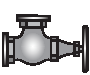
\includegraphics[scale=0.45]{../../figs/08HWEquivPipe/anglevalve} & Angle Valve & 150    \\
% 		\midrule
% 		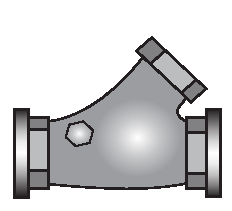
\includegraphics[scale=0.2]{../../figs/08HWEquivPipe/checkvalve}  & Check Valve & 100    \\
% 		\midrule
% 		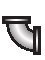
\includegraphics[scale=0.65]{../../figs/08HWEquivPipe/elbow}      & Elbow       & 50     \\
% 		\midrule
% 		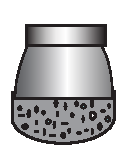
\includegraphics[scale=0.2]{../../figs/08HWEquivPipe/footvalve}   & Foot Valve  & 75     \\
% 		\midrule
% 		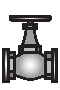
\includegraphics[scale=0.45]{../../figs/08HWEquivPipe/gatevalve}  & Gate Valve  & 35     \\
% 		\bottomrule
% 	\end{tabular}
% \end{textblock*}
%
%
% \begin{textblock*}{.35\textwidth}(13cm, 8cm)
% 	\centering
%
% 	\begin{tabular}{cccc}
% 		\toprule
% 		Pipe & Length (m) & diam (mm) & C   \\
% 		\midrule
% 		AB   & 10         & 500       & 125 \\
% 		\midrule
% 		BC   & 2000       & 275       & 150 \\
% 		\midrule
% 		BD   & 1500       & 250       & 100 \\
% 		\midrule
% 		DC   & 1000       & 300       & 100 \\
% 		\midrule
% 		CE   & 10         & 500       & 125 \\
% 		\bottomrule
% 	\end{tabular}
% \end{textblock*}
% %\begin{textblock*}{.6\textwidth}(2cm, 15cm)
% %\cbox{
% %\begin{itemize}
% %\item[] Diam of equiv pipe for BDC (series) = 217.91 mm
% %\item[] Diam of equiv pipe for BC (parallel) = 325.82 mm
% %\item[] Diam of equiv pipe for AE (series) = 324.98 mm
% %\item[] Q = 96.978 L/s
% %\end{itemize}
% %}
% %\end{textblock*}
% ~
% \vspace{13cm}
%
% \cmini[0.9]{
% 	\textbf{Solution}
% 	\parb
% 	\cbox{
%
% 		The objective is to replace the system of five pipes $AB,\,BC,\,CD,\,DC$ and $CE$ with a single hydraulically equivalent
% 		pipe from $A$ to $E$. Then we can use the Hazen-Williams equation to find flow through the system.\parb
% 		Our process will be as follows:
% 		\begin{enumerate}
% 			\item Find the effective lengths of the pipes that have valves or fittings.
% 			\item Consider the series system of two pipes $BD$ and $DC$: find a hydraulically equivalent pipe $BDC$.
% 			\item Consider the parallel system of two pipes $BDC$ (just found above) and $BC$: find a hydraulically equivalent pipe $BC2$
% 			      for flow from $B$ to $C$.
% 			\item Consider the series system of three pipes $AB,\,BC2,\text{ and }CE$: find a hydraulically equivalent pipe $AE$.
% 			\item Use the General Energy Equation and the Hazen-Williams equation to find $Q$.
% 		\end{enumerate}
%
% 	}
% }
% \vfill
% \cmini[0.9]{
%
% 	\cbox{
% 		\textbf{(1)} Find the effective lengths of the pipes that have valves or fittings.
%
% 		\begin{align*}
% 			L_{\text{eff}}     & = \text{Actual Length + Diameter}\times\left(\Sigma\frac{L_e}{D}\right) \\\\
% 			L_{\text{eff}(AB)} & = 10 + 0.5(75+50+100) = 122.5\,\text{m}                                 \\
% 			L_{\text{eff}(BC)} & = 2000 + 0.275(50+35+50) = 2037.1\,\text{m}                             \\
% 			L_{\text{eff}(BD)} & = 1500 + 0.250(150) = 1537.5\,\text{m}                                  \\
% 		\end{align*}
%
% 	}
% 	\parb
% 	\cbox{
% 		\textbf{(2)} Find a single equivalent pipe $BDC$ for the two pipes $BD$ and $DC$ in series.\parb
%
% 		Find the headloss between $B$ and $C$ for a flow of 100 L/s though $BD$ and $DC$, using the effective lengths of the pipes.
%
% 		\begin{align*}
% 			h_L        & = L\left(\frac{279000Q}{CD^{2.63}}\right)^{1.852}                                             \\\\
% 			h_{L(BD)}  & = 1537.5\left(\frac{279000\times 100}{100\times 250^{2.63}}\right)^{1.852} = 39.110\,\text{m} \\
% 			h_{L(DC)}  & = 1000\left(\frac{279000\times 100}{100\times 300^{2.63}}\right)^{1.852} = 10.467\,\text{m}   \\\\
% 			h_{L(BDC)} & = 39.110 + 10.467 = 49.577\,\text{m}                                                          \\
% 		\end{align*}
%
% 		\parb
%
% 		Find an equivalent pipe for $BDC$ (i.e., a pipe that has a head loss of 49.577 m for a flow of 100 L/s). We use an equivalent pipe with length 1000 m and resistance coefficient 100, and find the equivalent pipe diameter.
%
% 		\begin{align*}
% 			D       & = \left( \frac{279000Q}{C\left(\frac{h_L}{L}\right)^{0.54}}  \right)^{0.3802}                                      \\\\
% 			D_{BDC} & = \left( \frac{279000\times 100}{100\left(\frac{49.577}{1000}\right)^{0.54}}  \right)^{0.3802} = 217.92\,\text{mm} \\
% 		\end{align*}
%
% 	}
% }
% \cmini[0.9]{
%
% 	\cbox{
% 		\textbf{(3)} Now, consider pipe $BC$ and the pipe $BDC$ just found as a parallel system. Find an equivalent pipe for these two parallel pipes.\parb
%
% 		Assume a headloss of 10 m between $B$ and $C$ and find the flow through each of $BC$ and $BDC$:
%
% 		\begin{align*}
% 			Q                     & = \frac{CD^{2.63}\left(\frac{h_L}{L}\right)^{0.54}}{279000}                                      \\\\
% 			Q_{BC}                & = \frac{150\times 275^{2.63}\left(\frac{10}{2037.1}\right)^{0.54}}{279000} = 79.262\,\text{L/s}  \\
% 			Q_{BDC}               & = \frac{100\times 217.92^{2.63}\left(\frac{10}{1000}\right)^{0.54}}{279000} = 42.084\,\text{L/s} \\
% 			Q_{BC\text{ and }BDC} & = 79.262 + 42.084 = 121.35 \,\text{L/s}                                                          \\
% 		\end{align*}
%
% 		\parb
%
% 		A flow of 121.35 L/s between $B$ and $C$ through both pipes $BC$ and $BDC$ produce a headloss of 10 m. Find an equivalent pipe that replaces these two parallel pipes:
%
% 		\begin{align*}
% 			D_{BC\text{equiv}} & = \left( \frac{279000\times 121.35}{100\left(\frac{10}{1000}\right)^{0.54}}  \right)^{0.3802} = 325.83\,\text{mm} \\
% 		\end{align*}
%
% 	}
%
% }
%
% \cmini[0.9]{
%
% 	\cbox{
% 		\textbf{(4)} Now we have a series system: $AB,\, BC\text{equiv}$ and $CE$. Assume a flow of 100 L/s from $A$ to $E$, find the total headloss for this flow and then replace these three pipes with a single equivalent pipe.\parb
%
% 		\begin{align*}
% 			h_{L(AB)}             & = 122.5\left(\frac{279000\times 100}{125\times 500^{2.63}}\right)^{1.852} = 0.070450\,\text{m} \\
% 			h_{L(BC\text{equiv})} & = 1000\left(\frac{279000\times 100}{100\times 325.83^{2.63}}\right)^{1.852} = 7.0000\,\text{m} \\
% 			h_{L(CE)}             & = 10\left(\frac{279000\times 100}{125\times 500^{2.63}}\right)^{1.852} = 0.0057510\,\text{m}   \\\\
% 			h_{L(AE)}             & = 0.070450 + 7.0000 + 0.0057510 = 7.0762\,\text{m}                                             \\
% 		\end{align*}
%
% 		\parb
%
% 		Find the equivalent pipe that has a headloss of 7.0762 m for a flow of 100 L/s:
%
% 		\begin{align*}
% 			D_{AE} & = \left( \frac{279000\times 100}{100\left(\frac{7.0762}{1000}\right)^{0.54}}  \right)^{0.3802} = 324.99\,\text{mm} \\
% 		\end{align*}
% 	}
%
% }
%
% \cmini[0.9]{
%
% 	\cbox{
% 		\textbf{(5)} From the General Enery Equation (disregarding velocity head at $E$), headloss through the actual system is 6.7 m. We just need the flow that generates this headloss: \parb
%
% 		\begin{align*}
% 			Q_{AE} & = \frac{100\times 324.99^{2.63}\left(\frac{6.7}{1000}\right)^{0.54}}{279000} = 96.983\,\text{L/s} \\
% 		\end{align*}
%
%
% 	}
%
% }
%



\end{document}
